\chapter*{Introducci\'on}
\addcontentsline{toc}{chapter}{Introducci\'on}

\section*{Motivación}

Para el actual documento, las razones que motivaron al alumno presente a realizar la investigación de su tesis son la de comenzar a 
entrar en una rama que en los últimos años ha tomado bastante importancia en la informática, conocido como la {\textit{Bioinformática}} \cite{bioinformatica}, la cual aplica las tecnologías computacionales contemporáneas a datos biológicos que pueden pertenecer a estructuras como ADN, proteínas, entre otras estructuras biológicas complejas y los cuales están a la mano del ser humano como archivos de cadenas de secuencias (en varios formatos) y que pueden ser usados a voluntad.

En el caso puntual de esta memoria, se trabajarán con proteínas (compuestas de combinaciones de 20 aminoácidos) que están distribuidas en un {\textit{dataset}} cuyo formato del archivo está en \textbf{.fasta}, donde cada cadena de polipéptido está compuesto por un ID o código identificador, su nombre taxonómico y su posterior secuencia de aminoácidos. 


%\begin{figure}[H]
%\centering
%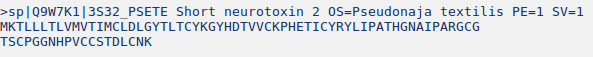
\includegraphics[width=14cm]{./images/cadena.png}
%\end{figure}

Hablando de las proteínas, se han realizado numerosos análisis \cite{searching, array} en bases de datos de secuencias con respecto a la cantidad de aminoácidos que se encuentran en total en este tipo de estructuras, distribuyéndolos según su tamaño o para determinar cuál es el aminoácido que más aparece en este tipo de archivos; también según el año de descubrimiento de las proteínas o el tipo de proteína. Todo esto usando fuentes como UniProt y EROP-Moskow. 

Como una derivación directa, existe una variabilidad casi infinita de combinaciones llamadas residuos (fragmentos) de aminoácidos ({\textit{amino acid residues}} o AAR de manera simplificada en inglés) que se determinan según su tamaño $k$ y por las posibles opciones a obtener, que sigue la regla de combinatoria $20^{k}$ ya que son 20 los animoácidos base que existen en la actualidad (para dipéptidos serían $20^{2} = 400$, para tripéptidos serían $20^{3} = 8000$ y así sucesivamente).